\documentclass{article}
\usepackage{algorithm}
\usepackage{algorithmic}
\usepackage{graphicx}
\begin{document}
\title{Specialized Cost Function for Maximizing Body Area Network Lifetime Using Global Routing Algorithms\\
Masters Thesis}
\author{Alvaro Prieto\\
BS/MS Electrical Engineering\\
\texttt{axp8664@rit.edu}}
\maketitle

\pagebreak

\tableofcontents

\pagebreak

\addcontentsline{toc}{section}{\protect\numberline{}Abstract}
\section*{Abstract}
Wireless Body Area Networks (WBANs) consist of several wireless sensors located around a human body. These sensors may measure several biological signals, movement, and temperature. Due to major improvements in power consumption and constantly shrinking devices, WBANs are becoming ubiquitous. As a side effect present because of the small form factor of these devices, the battery size is limited. While the sensors themselves may be extremely power efficient, all of the measured data must be transmitted over a much less efficient wireless link. One benefit of WBANs is that they rarely include more than a dozen wireless devices over a small area. This constraint allows for the use of routing techniques not suitable for larger wireless sensor networks(WSNs).

This work primarily focuses on maximizing the lifetime of WBANs. It also includes a basic software framework for developing WBANs, a sample Wireless Electrocardiogram (ECG) application, and a simple link cost algorithm development platform.

\section{Summary of Contributions}
The following is a list of contributions presented in this work.
\begin{itemize}
\item \textbf{Software platform for WBAN research.} - The software platform was developed using only free and open source software (FOSS) tools. Radio libraries for the Texas Instruments (TI) CC430 device were ported over from TI reference code, while libraries for the CC2500 radio were written from scratch. Other features include timer control for scheduling and time-stamping, serial communication, some digital I/O, and analog input. Included in the platform were limited software tools for data capture and visualization on a host computer.

\item \textbf{Wireless ECG platform} - In order to test and demonstrate the WBAN platform, a wireless ECG system was implemented. The system included three wireless devices, an access point, and a host computer. Software for synchronized sampling was developed and tested successfully using the WBAN platform. Three ECG leads were sampled at 300Hz and displayed on a host computer in real-time.

\item \textbf{Software platform for routing algorithm development} - In order to develop a novel routing algorithm, a platform to test and compare with others was developed. The application uses Dijkstra's algorithm for best path selection, and allows for the testing of various link-cost functions. Both simulation and real-time operation are supported. One unique feature is the generation of routing graphic generation for network visualization.

\item \textbf{Specialized cost function for maximizing WBAN lifetime using global routing algorithms} - A novel routing algorithm is developed that focuses not on single devices, but the network as a whole. Current methods focus on maximizing individual device lifetime or minimizing the energy-per-bit. While those are generally good goals, certain systems require all devices functioning to be considered operational. Keeping that in mind, the proposed system maximizes the network lifetime by normalizing power use across the network. For the purpose of this paper, \textbf{network lifetime} is defined as the time it takes any single node to deplete its energy source. 

\end{itemize}
% Include literature survey from other file
\section{Literature Survey}\label{section:litsurvey}
\subsection{Time Synchronization}
Time synchronization has been the subject of research for many years.

There are robust and time-tested synchronization methods, such as the Network Time Protocol (NTP)~\cite{synchronization:NTP}, which are currently in use around the world. Unfortunately these methods were designed for wired systems, and do not perform well once power consumption, latency, and other wireless effects taken into account. 

One of the first synchronization protocols designed specifically for wireless networks is Reference Broadcast Synchronization (RBS)~\cite{synchronization:RBS}. The main idea behind RBS is to synchronize all wireless sensor nodes to each other. This creates a local time, within the network of nodes, where all clocks are synchronized. For many applications, sensor nodes do not need to know the actual time, as long as they are synchronized to one another. \cite{synchronization:RBS} lists an example application that measures the time-of-flight of sound. If needed, RBS can be extended to use an external global time source to provide a relate the local and global times.

There are several sources of nondeterminism in a wireless network. ~\cite{synchronization:RBS} and ~\cite{synchronization:FTSP} decompose the sources of nondeterminism into several components. These components account for the delays due to the sending and receiving of a message in a wireless network. These components(from ~\cite{synchronization:RBS}) are: 
\begin{itemize}
\item \emph{Send Time} -- Time the sender takes to construct a message. Includes delays incurred by the operating system and time required to transfer the message from the host to the network interface.
\item \emph{Access Time} -- Time spent waiting for access to transmit channel.
\item \emph{Propagation Time} -- Time taken by the message to physically travel from sender to receiver.
\item \emph{Receive Time} -- Time spent processing a message and notifying the host of its arrival.
\end{itemize}

As suggested by its name, RBS uses broadcast messages to synchronize wireless nodes to one another. RBS does not synchronize a set of wireless nodes to a reference clock. Because of this property, RBS effectively eliminates the \emph{Send Time} and \emph{Access Time} as sources of error. The \emph{Access Time}, while unknown, is the same across all devices for any single message. RBS does not take \emph{Propagation Time} into account and considers it to be effectively zero. This is only a valid assumption if all nodes are equidistant from the broadcast message source. As stated in~\cite{synchronization:VHT}, the main benefit of RBS was due to high transmission nondeterminism. With new radio technology, this is no longer the main problem.

RBS is expandable for multi-hop networks, but has several requirements to do so. The first is that there must be multiple broadcast transmitters in order to cover the whole network. This creates several sub-networks of synchronized nodes, but does not synchronize them all together. The second requirement is that there must be a sort of overlap between broadcast transmitters. A sensor node receiving broadcasts from two different transmitters can compute the offset between the local times of both networks. 
\begin{figure}[htb]
\begin{center}
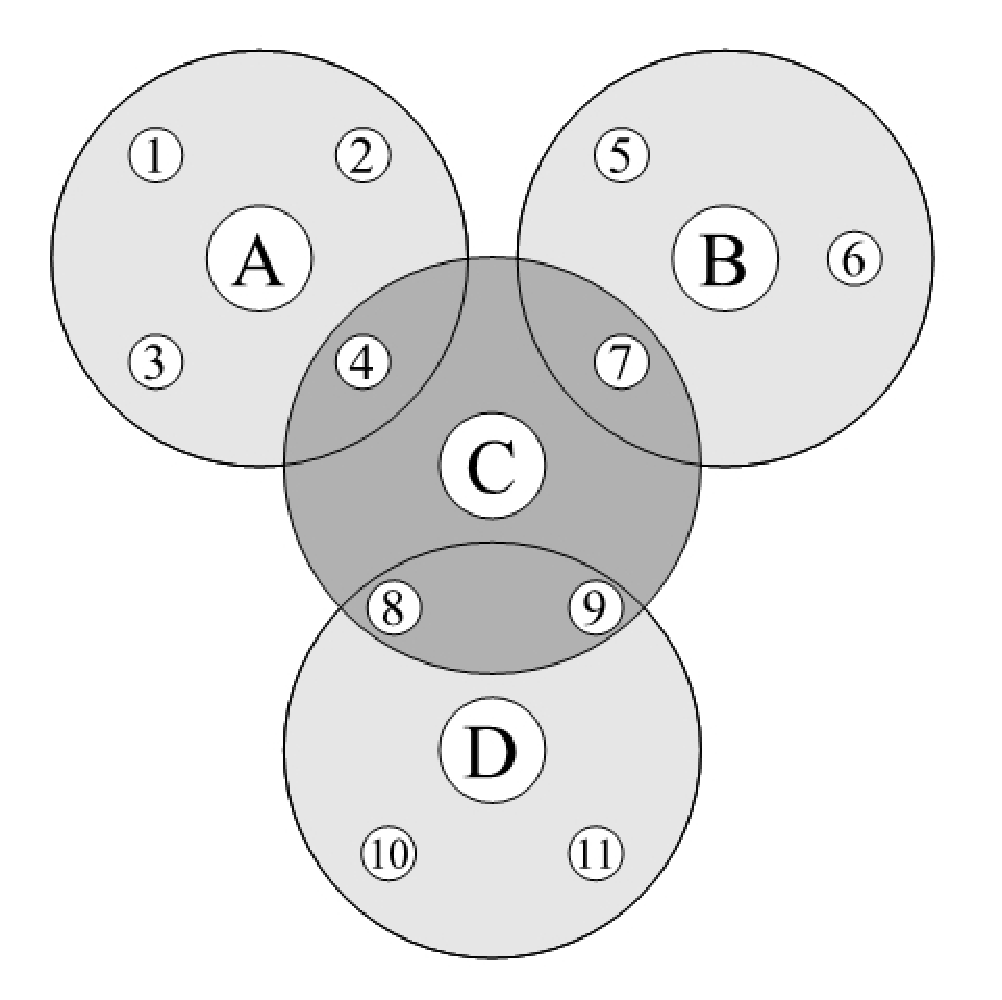
\includegraphics[width=0.4\textwidth]{figures/RBS_multihop.pdf}
\end{center}
\caption{RBS Multi-Hop Network Layout. From~\cite{synchronization:RBS}.}
\label{fig:RBS_multihop}
\end{figure}

Another time synchronization protocol introduced in~\cite{synchronization:TPSN} is the Timing-sync Protocol for Sensor Networks (TPSN). In contrast to RBS, TPSN synchronizes a set of notes to a single global time source. A hierarchical structure is established before synchronization can take place. Once the structure is in place, the root node begins to synchronize all nodes directly connected to it. Those nodes then do the same for their children nodes, etc...

TPSN utilizes the sender-receiver approach~\cite{synchronization:NTP} to synchronize a pair of nodes. A two-way message exchange provides enough information to calculate the clock difference and propagation delay between a pair of nodes. In order to synchronize the whole network, the root node initiates the process. In order to reduce packet collisions, each child node waits for a random amount of time before synchronizing to the parent. This is then repeated with the next level of nodes until they are all synchronized. Due to the very structured nature of TPSN, special protocols are provided for dealing with dying nodes, as well as newly introduced ones.

One of the costs of using TPSN over RBS is that the \emph{Send Time} is once again a source of error in the system. This is, however, mitigated by closely integrating TPSN at the Medium Access Control (MAC) layer. TPSN requires that both incoming and outgoing messages be timestamped at the MAC level in order to minimize uncertainties in transmit and receive times. 

The Flooding-Time Synchronization Protocol (FTSP)~\cite{synchronization:FTSP} is another protocol specifically designed for resource limited wireless platforms. Like TPSN, FTSP relies on MAC-layer time-stamping, along with several other new techniques, to synchronize devices. FTSP uses a single message to synchronize the clocks of to wireless nodes. By comparison, RBS uses a single message to synchronize the clocks of several devices to one-another, but not to the senders clock. TPSN uses two messages to synchronize two device clocks. Because of this, FTSP needs to account to other sources of error, such as the \emph{Byte Alignment Time}. All three protocols are susceptible to the jitter in \emph{Interrupt Handling Time}.

In FTSP, each device sends a broadcast message with its clock time. Devices in the vicinity listen to the broadcast and calculate the difference between their local and received times. In order to reduce jitter, FTSP records multiple times to compute a singe, more accurate time-stamp. This occurs on both the sending and receiving sides. 

Another important contribution from FTSP is a method to deal with clock drift. Due to differences in the exact frequency between local clocks, the time-difference between them grows over time.~\cite{synchronization:FTSP} proposes a solution that takes place off-line. In the short-term, the clock drift is fairly linear. Because of the linear fashion of clock drift, linear regression can be used to distribute the error over a period of time. If clocks are being synchronized every \emph{X} seconds, and clocks drift some amount \emph{Y}, the algorithm distributes the drift \emph{Y} over all samples in a \emph{X} second interval. The reason this must be done off-line is because \emph{Y} can only be computed after each synchronization. 

FTSP scales well to multi-hop wireless networks. Reference points are utilized to keep track of the time differences between the root node and the local node. FTSP is also resistant against losing nodes as it includes root  re-election protocols in case the root node fails. According to ~\cite{synchronization:VHT}, FTSP is currently the \emph{de facto} time synchronization protocol in wireless sensor networks.

The Gradient Time Synchronization Protocol (GTSP)~\cite{synchronization:GTSP} focuses on synchronization of close-by nodes in multi-hop networks. If two physically nearby nodes are part of two different synchronization trees, their clocks might be different. GTSP uses radio broadcasts overheard from all neighbors in order to provide a more accurate time in relation to close-by nodes.

There are certain disadvantages to each of these methods. RBS requires additional messages for time synchronization across multi-hop networks. TPSN does not account for the clock drift of sensor nodes. Both RBS and TPSN are vulnerable to jitter in interrupt handling and decoding times. While FTSP accounts for interrupt handling jitter, it does not take propagation time into account. This is not a problem if nodes are physically close, but can affect performance in long distance cases. GTSP and RBS are also vulnerable to propagation delay errors.

\subsection{Synchronized Sampling}
There are several applications, such as monitoring an active volcano ~\cite{applications:volcano}, structural monitoring~\cite{applications:structural} and counter sniper systems~\cite{applications:sniper}, which rely on synchronized measurements across sensor networks. Currently there is not much research focusing specifically on synchronized sampling in low-power WSNs. Apart from ~\cite{sampling:earthquake}, most research utilizes the previously described time synchronization protocols to keep device clocks aligned. With synchronized clocks, synchronized sampling is no longer a complex problem.

\subsection{Routing and Relaying}
Due to power and physical constraints, sensor nodes placed along the body may not be able to communicate with the main node directly. Even when sensor nodes are able reach the main node, the power required to do so could be prohibitive. The use of relays to re-transmit the data has been shown to dramatically reduce power consumption in body sensor networks~\cite{relay:creepingwave}.

There are several routing protocols currently used in WSNs~\cite{survey:wirelessrouting}, unfortunately, most are not well suited for BSNs. Several of the protocols focus on mobility, Quality of Service (QoS), scalability and reliability, among other things. In general, BSNs do not have the same requirements as other WSNs. For example, in BSNs, scalability is no longer a problem since networks are limited to a human body. In most cases, power consumption becomes the main limiting factor for overall system performance. 

Some routing protocols are specifically designed with BSN constraints in mind. One example is the Wireless Autonomous Spanning tree Protocol (WASP) \cite{protocol:WASP}. Braem et al. describe the WASP as ``a slotted protocol that uses a spanning tree for medium access coordination and traffic routing''. The main idea is that each node sends a ``WASP-scheme'' through a broadcast message that both parent and children nodes receive. This scheme contains the time allotments for each node for the current time frame. The children of the current node need the scheme to know when they are allowed to transmit data. The scheme also informs the parent of the current node as to how many children each node has, which allows it to allocate enough time slots for that branch. This method allows for a distributed time-allocation protocol. Each time frame also includes contention periods where new nodes can join the network. Routing is simple as data from sensor nodes is just sent up the network tree and broadcast messages are used to send configuration down from the root node. The main disadvantage of the WASP is the need to send the scheme packets from the root node down the tree during every time frame.

An improvement over the WASP is the Cascading Information retrieval by Controlling Access with Distributed slot Assignment (CICADA) protocol~\cite{protocol:CICADA}. The improvement over the WASP has to do with the separation of control and data subcycles. The WASP re-configures the time slots during every frame, which produces a significant time delay. The information has to move from the root node to all the children and back. The CICADA protocol configures the network in a separate subcycle and later transfers data. The data transfer is initiated from the bottom of the tree, so there is no delay waiting for the root node to send configurations down during each data subcycle.

Other BSN routing methods focus on postural mobility~\cite{routing:storeandforward}. Quwaider et al. propose a protocol tolerant to constant network changes due to body/sensor movement. When sensor nodes are located in body extremities, the wireless links vary with body position changes. The proposed protocol uses a store-and-forward method to transfer data from sensor nodes to the main node. While the protocol is well suited for dealing with mobile nodes, it requires more energy to do so. ``Hello'' packets are constantly sent by each node to determine what the current neighboring nodes are. A neighbor table is generated using this information and is necessary to determine where packets will be sent to. Another problem with the method is due to multiple copies of packets being transmitted to increase the probability of delivery. Finally, the main node transmits at full power in order to poll each sensor node, increasing its energy consumption.

Most current routing methods for BSNs use network trees. One of the main problems present with network trees is that the nodes closer to the main node deplete their energy supply faster than children nodes. This is due to the fact that all trafic from children nodes has to be relayed through. Ehyaie et al. propose using dedicated relay nodes instead of having sensor nodes act as relays~\cite{relay:networklife}. Using dedicated relays increases the individual sensor life, with the added cost of more devices.

So far, most BSNs have used tree-like networks to join nodes together. Tree networks, while simple, are negatively affected by node failures and movement.  Nabi et al. use a gossiping data routing strategy along with TDMA based MAC to transmit information to the main node \cite{relay:transmitpoweradaptation}. Each node receives and stores the last sample data from every neighboring node. During transmission, it sends its own sampled data, along with one or more of the stored packets from other nodes. This method maximizes the likelihood of a packed reaching the main node, while consuming more power due to retransmissions of the same data. Timestamps are used to decide whether or not a received packed will be stored or discarded. The main node is assumed to have higher battery capacity and transmission range. It is required to be able to reach all nodes with a single transmission. It is in charge of sending a synchronization beacon to use as a time reference for TDMA frames. This method is not always feasible, for example, when two nodes are on opposite sides of the body.

Another valuable contribution from~\cite{relay:transmitpoweradaptation} deals with Transmit Power Adaptation (TPA). The goal for TPA is to minimize power consumption while maintaining a specific link quality. It achieves this goal by adjusting Tx power according to link quality. Unlike the link quality metric in ~\cite{routing:storeandforward}, which was bidirectional, nodes have both inlink and outlink qualities. The outlink metric is then maintained within predefined thresholds by varying Tx power. Inlink quality is stored and later transmitted in order to share the information with neighboring nodes.

\subsection{Similar Work}
In order to determine the improvements of novel methods, reference systems need to be available to compare with. Both~\cite{mac:tdma}~and~\cite{mac:lowdutycycle} provide a suitable reference system for a synchronized, non-relaying BSN. Both proposed systems present, in detail, a TDMA MAC protocol specifically designed with energy efficiency in mind. Details of packet format, TDMA frame calculation, and power consumption measurements are available.
%Add more details later


%[The current system is further simplified by the complete determinism of network traffic. Each sensor node is continuously sampling data at a known rate and sending it back to the main node at known intervals. This allows for protocol simplifications and other energy saving things EXPLAIN!!! ]
 %uncomment to include literature survey


\section{Software Libraries}\label{sec:wbansoftwarelib}
One of the primary contributions of this project consists of software libraries for working with WBANs. Due to the project requirements, a choice was made to use free and open source tools, as opposed to proprietary software. Because of this choice, most of the radio libraries had to be either ported or re-written from scratch. There were two main hardware devices that were targeted in these libraries. The first consisted of a CC430 device, which has a built in 915MHz radio. The second was an MSP430 with an external CC2500 2.4GHz radio.

\subsection{Project History}
The first software libraries were initially developed by Corey Provencher, a student at RIT, for a senior design project. He developed a hardware board with a variety of sensors to measure body movements and the corresponding software to use it. All of his software development was done using the Texas Instruments (TI) software tools on Windows(TM).

Jeffery Robble, another student, took over and ported most of the code to use Linux based open source tools. The code ported over by Robble used TI's radio stack \emph{SimpliciTI}. Unfortunately, SimpliciTI was too complex and resource heavy to do time-sensitive operations, like clock synchronization, over the radio. It also required the use of other TI software libraries in order to work.

After Robble left, the work continued. The main goal of the project at the time was to develop wireless electrocardiogram(ECG)(Section~\ref{section:wirelessecg}). While planning for the wireless ECG, a decision was made to develop an entire WBAN platform that could later be used for other projects. The new platform would be developed in-house and included both hardware and software. Because of this, the entire library was to be written from the ground up. This would prevent any rights issues from coming up if published.

\subsection{Design Choices}
The decision to write all software libraries from scratch was not an easy one. Initially the SimpliciTI libraries were modified to try and meet the project needs, but this proved to be a complex task. Due to the simple nature of the planned WBAN, a much less complex approach could be used. The main application only required streaming data from various wireless sensors.$\ll$ Should I elaborate on the design constraints here? The number of devices is known, the time of transmission is known etc...$\gg$ This could be accomplished with a very minimal radio library.

\subsection{CC430 Device}
The first device used in this project was Provencher's initial hardware platform. Due to the limited quantities of that device, a new version of the hardware platform was developed. The new device removed all unused sensors from the board to minimize its footprint. It included a CC430 device with a 32.768Khz crystal oscillator for precise timekeeping. The analog-to-digital(A/D) ports were used to attach any needed sensors. The actual CC430 model used was the CC430x6137.

Libraries were written for serial communication, visual indicators, analog measurements, time synchronization and radio communications. The serial communication was used to transmit data to the host computer, while the rest were used in the wireless ECG application.

\subsection{MSP430-RF2500 Device}
The second major hardware platform was the MSP430-RF2500. This device is manufactured by TI and sold as a development platform. The MSP430-RF2500 device consists of an MSP430F2274 microcontroller and a CC2500 radio. There were several reasons why this device was used. The primary use for the MSP430-RF2500 was to develop the libraries to use the CC2500 radio. The next planned hardware platform for the project consisted of a CC430 with a CC2500. The previous software libraries would need to be expanded to include a second radio for communication.

Unlike the CC430, which has a radio core built in, the CC2500 is a standalone unit. In order to expedite the software development process, a working platform was needed. Software development new, untested, hardware is not a feasible option. Debugging both hardware and software simultaneously is not a good idea.

The previously developed CC430 libraries were ported to work with the MSP430 microcontroller and expanded to use the CC2500 radio. Features of the new radio libraries include power control, addressing and channel switching.

\begin{figure}[htb]
\begin{center}
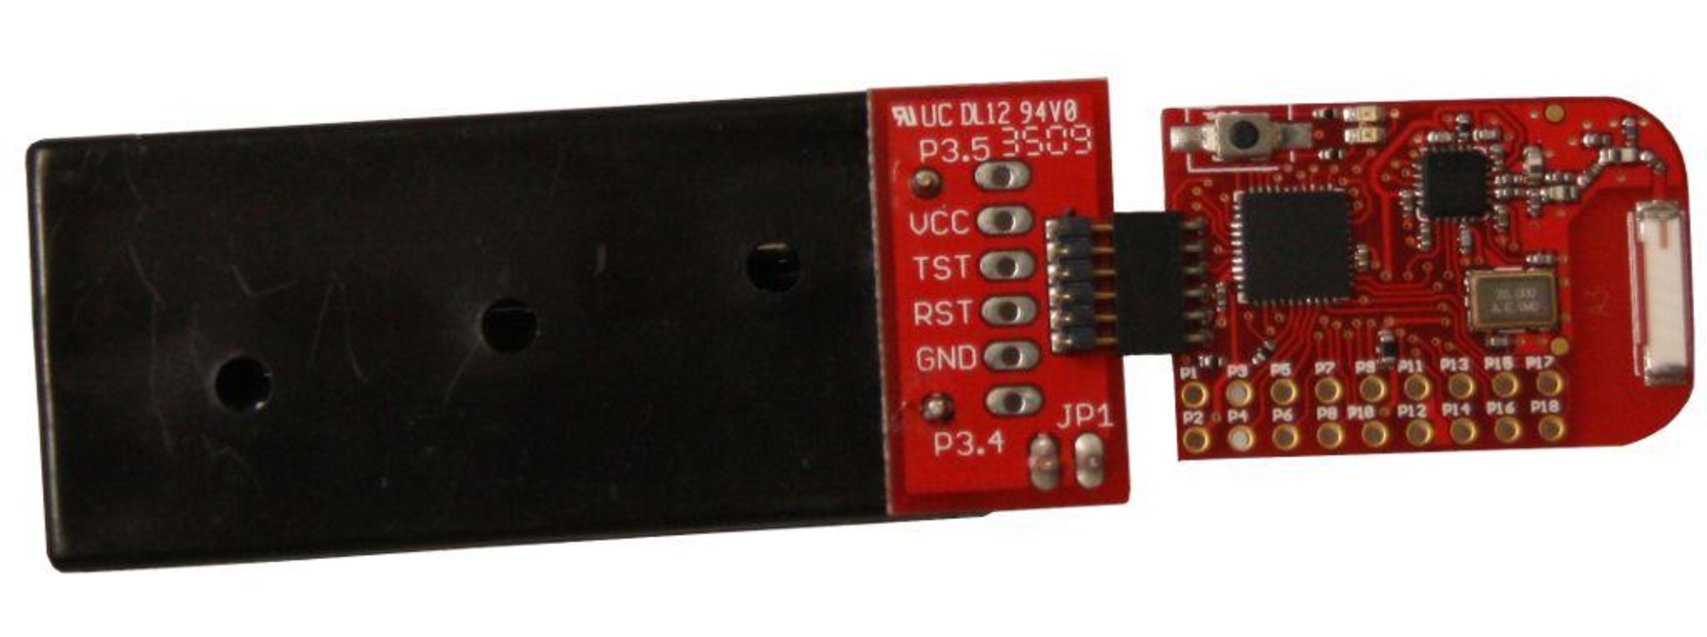
\includegraphics[width=0.9\textwidth]{figures/ez430-rf2500.pdf}
\end{center}
\caption{EZ430-RF2500 with Battery Pack}
\label{fig:ez430}
\end{figure}

\section{Wireless ECG Application}\label{section:wirelessecg}
\subsection{Description}
The main goal of the Wireless ECG application is to produce the equivalent output of a traditional, wired, 12-lead ECG using three wireless sensors. 

The three main parts of the wireless ECG project are: 
\begin{itemize}
\item Developing the analog front-end to measure the biopotential signals from the subject.
\item Developing the software/firmware libraries to measure, store, and transmit the data from the EDs to the host.
\item Developing the lead reconstruction algorithms to convert the 3 measurements back to a physician friendly 12-lead display.
\end{itemize}
The work presented here focuses on the software/firmware development for the application.

\subsection{TinyOS Platform}
The first wireless ECG platform was developed using the Imperial College London BSN Motes, which use the TinyOS operating system. These devices are programmed in a derivative of the C language called NesC. While working with these devices and operating system was not particularly simple, the hardware worked, and had been used in other projects. A full 3-sensor wireless ECG application (minus the lead reconstruction) was implemented with these devices. Since the devices run an operating system, several, non-ideal, modifications were required to obtain precise time synchronization.

\subsection{CC430 Platform}
After demonstrating the system using the TinyOS devices, the development of the in-house system continued. After several hardware implementations, a similar 3-sensor wireless ECG application was developed. In contrast to the TinyOS system, the CC430 platform only used hardware and software that was developed by the team.

\subsection{Time Synchronization}
The method used compensates for time offsets between samples and minimizes the effect of clock drift by periodically synchronizing independent clock sources together. Figure~\ref{fig:network_layout} shows an example system consisting of three end devices (\emph{ED}s), one access point (\emph{AP}) and one host computer. 
\begin{figure}[htb]
\begin{center}
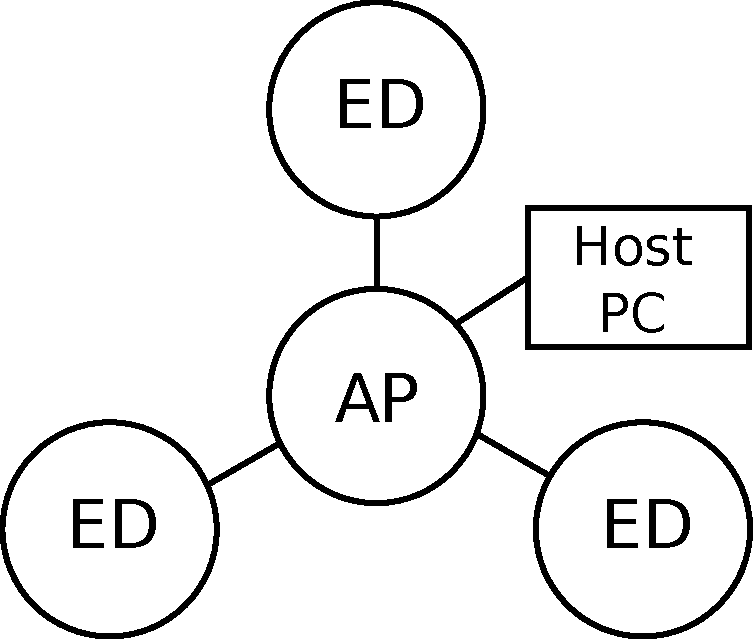
\includegraphics[width=0.4\textwidth]{figures/network-map-test2.pdf}
\end{center}
\caption{Test Network Layout}
\label{fig:network_layout}
\end{figure}
All devices have a timer used for time-stamping and synchronization. All events, including samples and data transfers, occur according to the value of the timer. Due to certain hardware limitations, the value of the timer cannot be altered, it can only be reset to zero. This does not, in any way, affect the synchronization of devices.

The timer inside the \emph{AP} can be considered the primary, or global, timer. The goal is to synchronize all \emph{ED}, or local, timers with the global timer. Whenever the global timer reaches its maximum value, and rolls over back to zero, the \emph{AP} sends a broadcast synchronization beacon instructing each end device it is time zero. When an \emph{ED} receives this message, it compares its current timer value to zero, to calculate the clock drift, and resets it to zero. This ensures that all \emph{ED} timers are aligned, which then allows measurements to occur at close to the same time.

While many, more precise, time synchronization methods are available~\cite{synchronization:FTSP}, it was determined that they were not needed. Due to the low sampling rate and the use of crystal oscillators to run the timers, the precision obtained with this simple method was good enough for the system. More complex methods would not have significantly improved results. Figure~\ref{fig:sync_data} shows the result of three separate wireless devices measuring the same signal. This method was used to confirm that the samples were aligned.

\begin{figure}[htb]
\begin{center}
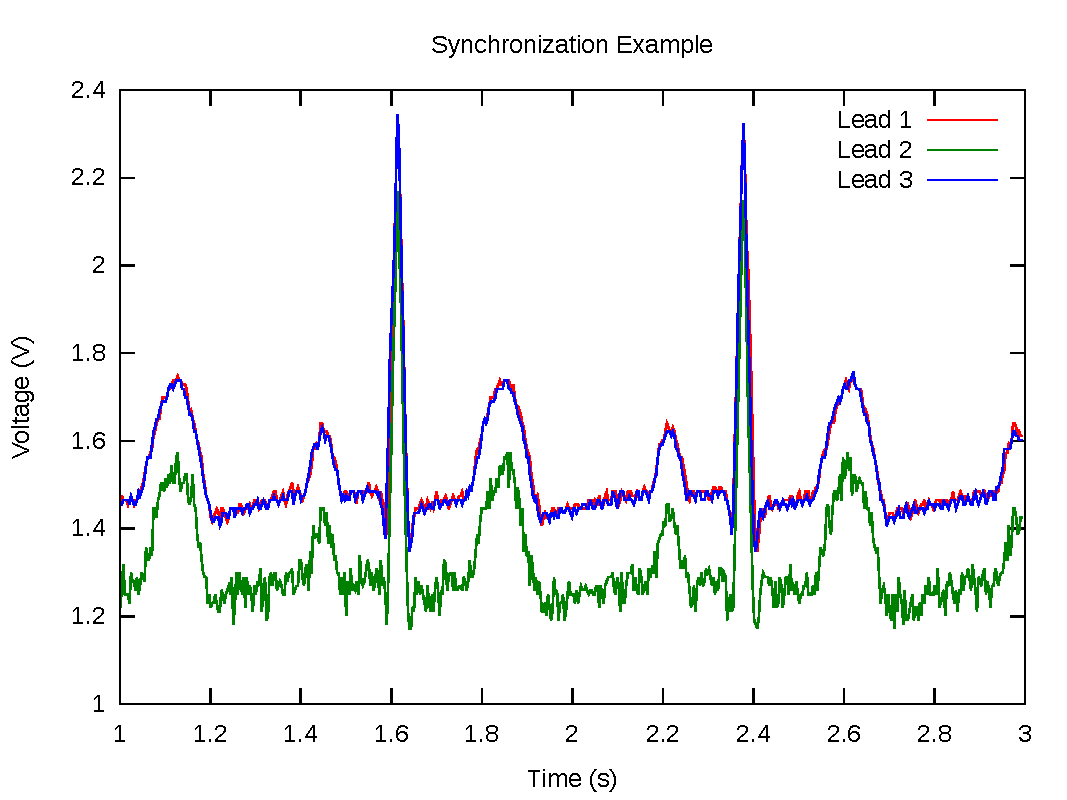
\includegraphics[width=0.8\textwidth]{figures/syncdata.pdf}
\end{center}
\caption{Synchronization Test}
\label{fig:sync_data}
\end{figure}

\subsection{Scheduling}
A round robin-like scheme is used to poll devices in the network. It focuses on simplicity and portability.

In previous implementations, each \emph{ED} was polled individually for sampled data, which required all \emph{ED}s to be on at all times. Once all device clocks are synchronized, polling is no longer necessary. Instead of sending poll messages to each device, the \emph{AP} just listens for \emph{ED} transmissions. The \emph{ED}s will wake up when they are scheduled to transmit and send the required data automatically. This method greatly reduces the power consumption of both \emph{AP} and \emph{ED}s. After initialization, the \emph{AP} only needs to send a periodic time synchronization beacon and the collected data back to the host computer. Once synchronized, end devices will only need to turn their receiver on around the time the synchronization beacon is expected.

Figure~\ref{fig:system_schedule} shows a sample system schedule. The figure shows the time each device is on, and the state of each radio. The ``sleep'' time for each \emph{ED} does not show when a device wakes up to sample data. In this specific case, the \emph{AP} has one extra time-slot allotted for a fourth \emph{ED}.

\begin{figure}[htb]
\begin{center}
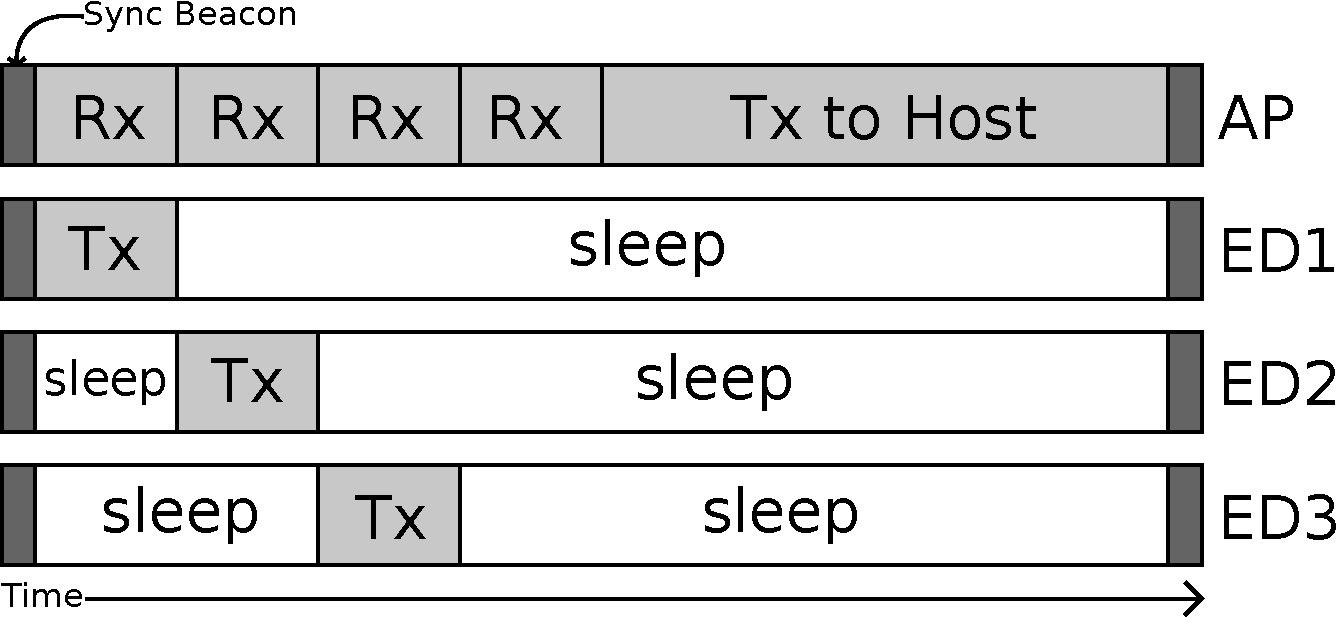
\includegraphics[width=1\textwidth]{figures/sync_schedule.pdf}
\end{center}
\caption{System Schedule}
\label{fig:system_schedule}
\end{figure}

Certain devices can further reduce power consumption by sampling without using the main processor. This works by using direct-memory access(\emph{DMA}) which allows the analog-to-digital converter(\emph{ADC}) to store measurements in memory without first going through the processor. Using this method, Figure~\ref{fig:system_schedule} accurately presents the time each \emph{ED} is powered on. Sampling with DMA has not been implemented in the current wireless ECG platform.

\begin{figure}[htb]
\begin{center}
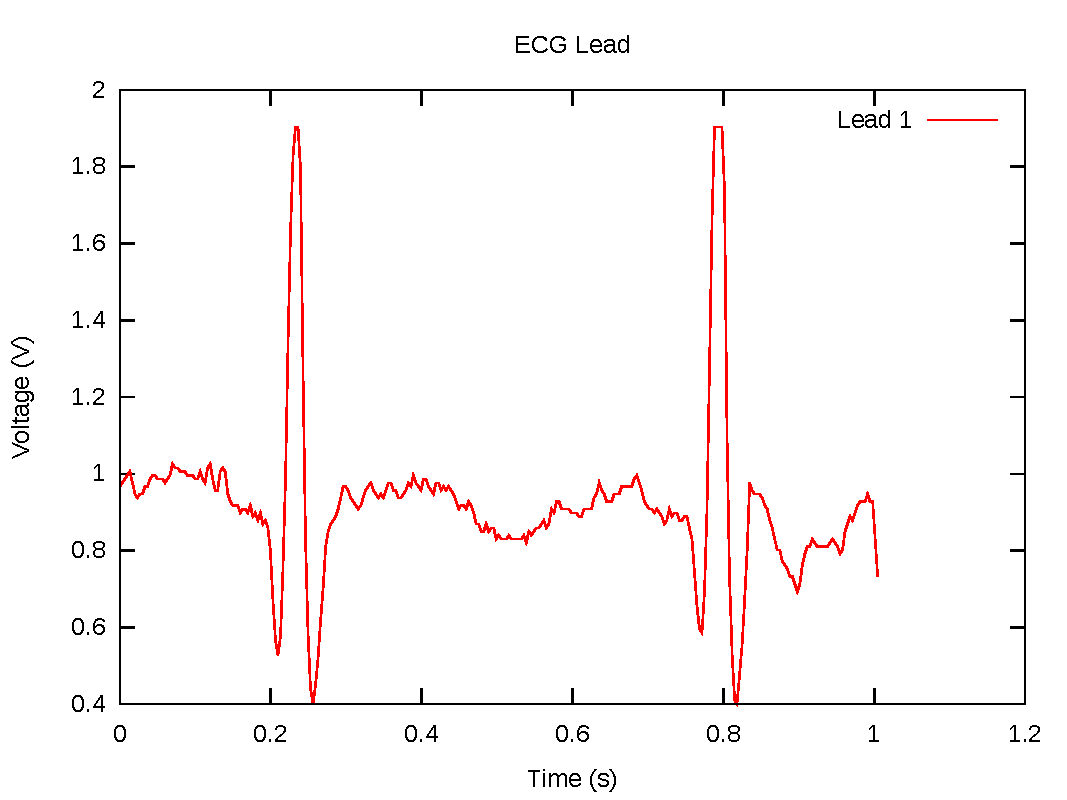
\includegraphics[width=0.8\textwidth]{figures/heartbeats.pdf}
\end{center}
\caption{Sample Measurement from Single ECG Lead}
\label{fig:heartbeats}
\end{figure}

\subsection{Host Interface}
The primary focus of this project was to obtain synchronized samples from several wireless devices. A secondary, but important, goal was to display the data in real time. To speed up development, the live-plotting tool kst(http://kst-plot.kde.org/) was used. A application, written in C, communicated via a USB-to-Serial link with the AP and received all of the ED data. It then output the data to CSV files, which were then used as an input for kst. Figure~\ref{fig:heartbeats} shows an ECG lead wirelessly measured from a human subject.



\section{Algorithm Development Platform}
A platform for testing and analyzing new cost functions for global routing algorithms was developed in C. The platform allows for a network of nodes and links between the nodes to be created. It computes the best path from any node to a central source node. Finally, it produces various statistics, such as energy use, routing maps, and graphical visualizations.

\subsection{Initial Development}
Initially, the goal of the platform was to test and compare routing with various link costs in an efficient manner. After a good link cost function was found, it would then be implemented in a microcontroller and used. This did not turn out to be the case. The first problem encountered dealt with the network structure used for testing. The program required a list of nodes and a list of links between the nodes, along with the link costs. Developing a simulated network and links that accurately represented a real network was unfeasible. The choice was then made to closely couple the hardware design and the simulator.

\subsection{Hardware Coupling}
The best way to come up with a network for simulation was to get all of the node and link information from a real network. The WBAN platform was then used to develop a system for measuring RSSI data between all nodes in a network. This system allowed for the capture of real network data, both nodes and links, that could later be used to run routing simulations. The new program auto-generated a list of nodes, links, and link costs from the previously-measured RSSI data. This new approach effectively removed the need to come up with special networks for testing. 

\subsection{Simulation Output}
In order to better understand how the new routing system performed, a series of output files were generated during simulation. The program was set up to account for the energy use of each node as it routed packets through the network. Visualizing the energy use was vital for the analysis of network lifetime. Other available data included the routing information itself, which allowed for the analysis of the routes as the algorithm runs. During run-time, the program prints out text-based routing information in a terminal window(Figure~\ref{fig:textoutput}). This provided real-time feedback that was useful during hardware debugging.

\begin{figure}[htb]
\begin{center}
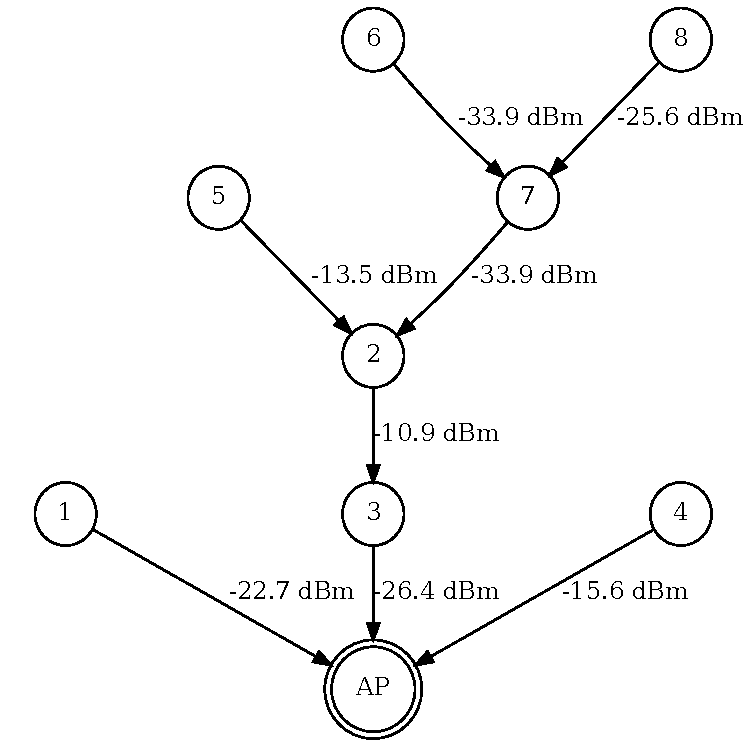
\includegraphics[width=0.6\textwidth]{figures/networkgraph1.pdf}
\end{center}
\caption{Sample Network Visualization}
\label{fig:networkgraph1}
\end{figure}

Finally, the program produced a graphical output. The graphical output began as a simple experiment to see a visual representation of the network. It was later expanded to generate graphs of the network, and all available connections, as the RSSI data was sampled. Due to the large number of links between all of the nodes, this graphic was not useful. The final implementation, which can be seen in Figure~\ref{fig:networkgraph1}, only displayed the links used in a specific round of routing. The link labels display the transmit power required by each node to meet the specific link. The generated graphs can later be put together to form an animation that shows the network changing in action.

\begin{figure}[htb]
\begin{center}
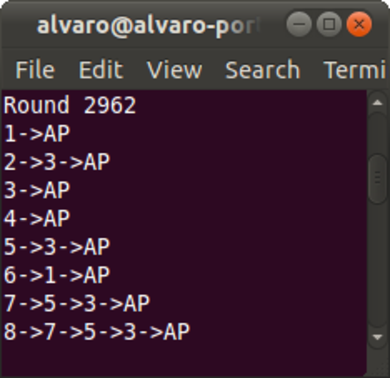
\includegraphics[width=0.5\textwidth]{figures/textoutput.pdf}
\end{center}
\caption{Sample Run-time Output}
\label{fig:textoutput}
\end{figure}



\section{Specialized Cost Function for Maximizing Body Area Networks Lifetime Using Global Routing Algorithms}\label{sec:costfunction}
\subsection{Introduction}

There are several routing protocols designed specifically for WBANs. Braem et al. developed the CICADA protocol, which consists of a spanning tree architecture with a time-division scheme for transmission scheduling~\cite{protocol:CICADA}. The primary downside to this method is that nodes closer to the root will deplete their energy source faster due to the need to relay messages from children nodes. Other protocols focus on the reliability of the network~\cite{routing:storeandforward}. Dynamic networks are a problem with WBANs. If sensors are placed in the extremities, the network will change as the body changes positions. Quwaider et al. developed a protocol tolerant to network changes~\cite{routing:storeandforward}. They propose a store-and-forward method that maximizes the likelihood of a packet reaching its destination. Each packet is stored by multiple devices and retransmitted, which consumes more power. One solution for this problem was proposed by Ehyaie et al.~\cite{relay:networklife}, it consists of using dedicated, non-sensing, relay nodes with larger power sources. While this method increases the network lifetime, it requires more hardware. Finally, Nabi et al. propose a similar store-and-forward method, but integrates Transmit Power Adaptation (TPA)~\cite{relay:transmitpoweradaptation}. Nodes keep track of neighbors and use power control to use the smallest transmit power while maintaining a specific link quality.

In order to provide accurate channel conditions, RSSI measurements of an eight ED network were used as input to our simulations(\ref{sec:simulation}). Real-time hardware implementations were also run to demonstrate the algorithm(\ref{sec:hardware}). The new cost function succeeded in improving network lifetimes when run in a dynamic environment. Static environments did not produce successful results.

\begin{figure}[!htb]
\begin{center}
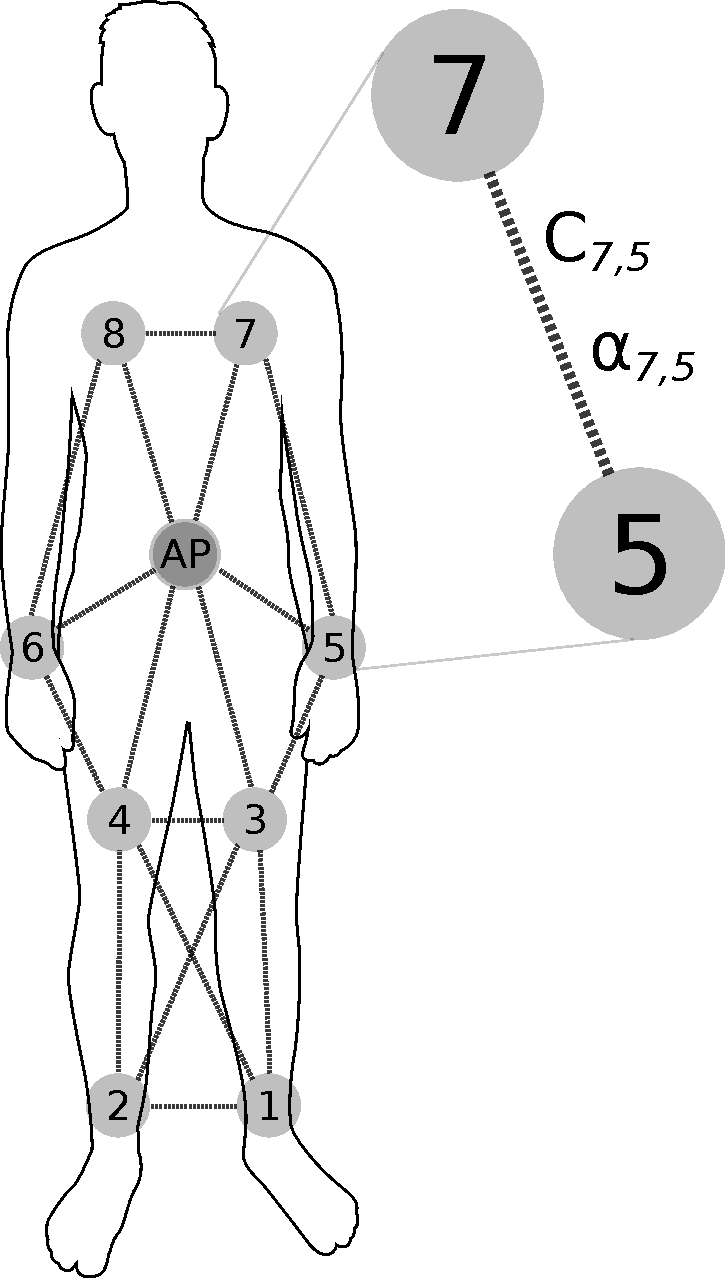
\includegraphics[width=0.5\textwidth]{figures/body.pdf}
\end{center}
\caption{Experimental Setup (Not all links shown)}
\label{fig:body}
\end{figure}

\subsection{Proposed Cost Function}
In the proposed system, we define a new link cost function that is then used in a routing algorithm. Traditionally, the power required to make a link possible is used as the link cost. In this case, the total energy used by a device is factored into the equation. If a device has used more energy than the others, its use as a relay will be discouraged.

\subsubsection{Device Energy}
Each device's normalized energy use is calculated as shown in Equation~\ref{eqn:accumulated_energy}, where $j$ denotes the device ID, $i$ is the current polling round, $\alpha_{j,k}$ is the channel attenuation for the selected link, and $RSSI^T$ is the target RSSI. The current energy used is incremented by the energy used to transmit a single packet while maintaining $RSSI^T$. The channel attenuation for the selected link,$\alpha_{j,k}$, can be seen in Equation~\ref{eqn:alpha}, where RSSI is the received power measured by device $k$ and $P_{tx}$ is the transmitted power used by device $j$. 

\subsubsection{Link Cost}
The actual link cost is computed by calculating the energy used by the device, \emph{if} that link is selected, and multiplying by a cost factor(Equation~\ref{eqn:link_cost}). The cost factor calculation takes the energy used by the destination device, $E^k_i$, and divides it by the current energy minimum, $E^{min}_{i}$, which is the energy used by the device with the minimum energy used by round $i$. This ratio is then raised to the power $M$, which determines how strong the effect will be. If a device's energy is much greater than the current minimum, it will be avoided as a relay.
The $M$ factor in Equation~\ref{eqn:link_cost} can be any number in $0 < M < \infty$. The cost factor is normalized so when $M=0$, it returns to the traditional cost of required power to meet the link.

Since the link costs are directly related to the destination device, they are calculated during the routing algorithm computation. For this paper, Dijkstra's algorithm~\cite{dijkstra:algorithm} is used to select the best route.

\begin{equation}
\label{eqn:alpha}
\alpha_{j,k} = \frac{RSSI}{P_{tx}}
\end{equation}
\begin{equation}
\label{eqn:accumulated_energy}
E^j_{(i)} = E^j_{(i-1)} + \frac{RSSI^T}{\alpha}
\end{equation}
\begin{equation}
\label{eqn:link_cost}
C^i_{j,k} = \frac{RSSI^T}{\alpha_{j,k}} \times \left( \frac{1+\left(\frac{E^k_i}{E^{min}_{i}} \right)^M}{2} \right)
\end{equation}

\subsubsection{Assumptions}
This algorithm works under several assumptions. The first being that this is a centralized network with one Access Point (AP) with virtually unlimited energy and computing power. The second is that each wireless sensor, or End Device(ED), can act as a relay for messages from other nodes. The Third is that the link quality, or channel attenuation, between all EDs and AP is known. Finally, all EDs begin with an equal energy used, that is, they all have the same energy stored. All routing calculations take place in the AP. Figure~\ref{fig:body} shows a sample network with EDs labeled 1 through 8, and one AP.

\subsection{Performance Analysis}
In what follows, we analyze the performance of the proposed cost function. The new cost function was tested in both simulated and experimental environments. In order to gauge the efficiency of the cost function, it will be compared to an identical system which uses a traditional link cost function. The traditional link cost function consists of the required power to meet a link with the desired $RSSI^T$. This can be achieved by setting a value of $M=0$ in the new link cost function.

Performance is determined by the time it takes any node's accumulated normalized energy to cross an arbitrary threshold. The threshold could be equivalent to the amount of energy stored in a device battery, but for this experiment, is purely arbitrary. 

\subsubsection{Algorithm Implementation}
Detailed pseudo-code for the routing algorithm can be found in Algorithm~\ref{alg:dijkstra}. Similarly, code for energy used calculation can be found in Algorithm~\ref{alg:energyused}.

\begin{algorithm}[!ht]
\caption{Dijkstra's Algorithm with new cost function}
\label{alg:dijkstra}
\begin{algorithmic}[1]
\FOR{$i = 1$ to \# of Nodes} 
	\STATE $node_i.visited \leftarrow 0$
	\STATE $node_i.distance \leftarrow \infty$
	\STATE $node_i.previous \leftarrow node_i$
\ENDFOR
\STATE $node_{AP}.distance \leftarrow 0$
\STATE $energy_{min} = min(node.energy)$
\WHILE{unvisited nodes available}
	\STATE $node_{source} \leftarrow $ node with smallest distance
	\FOR{$i = 1$ to \# of Links}
		\IF{$link_i.source = node_{source}$}
			\STATE $node_{dest} \leftarrow link_i.destination$
			\IF{$node_{dest}.visited = 0$}
				\STATE $cost \leftarrow link_i.power * (1 + node_{dest}.energy/energy_{min} )^M/2$
				\STATE $newdistance \leftarrow node_{source}.distance + cost$
				\IF{$distance < node_{dest}.distance$} 
				\STATE$node_{dest}.distance \leftarrow newdistance$
				\STATE$node_{dest}.previous \leftarrow node_{source}$
				\ENDIF
			\ENDIF
		\ENDIF
	\ENDFOR
	\STATE $node_{source}.visited \leftarrow 1$
\ENDWHILE
\end{algorithmic}
\end{algorithm}

\begin{algorithm}[!ht]
\caption{Energy Used Calculation}
\label{alg:energyused}
\begin{algorithmic}[1]
\FOR{$i = 1$ to \# of Nodes}
	\STATE $node_{ptr} = node_i$
	\IF{$node_{ptr}.previous = node_{ptr}$}
		\STATE No path to $node_i$
	\ELSE
		\WHILE{$node_{ptr}.previous \neq node_{ptr}$}
			\STATE $link_{ptr} \leftarrow $ link between $node_{ptr}$ and $node_{ptr}.previous$
			\STATE $node_{ptr}.energy += link_{ptr}.power$
			\STATE $node_{ptr} \leftarrow = node_{ptr}.previous$
		\ENDWHILE
	\ENDIF
\ENDFOR
\end{algorithmic}
\end{algorithm}


\subsection{Simulation}\label{sec:simulation}
In order to test the new cost function in an efficient manner, a simulation was used. Measurements of real channel data were acquired by running the procedure described in~\ref{subsec:cycleofoperations} without the routing or power control enabled. Each ED continuously sampled RSSI data from all other devices and transmitted it to the host. 

Two experimental setups were used to capture RSSI data. For the first, the subject(See Figure~\ref{fig:halfbody}) remained relatively static in a sitting position. The second consisted of a more dynamic environment, where the subject walked around a room as seen in Figure~\ref{fig:floorplan}. 

A set of captured RSSI tables (as seen in Table~\ref{tab:rssi}) were fed into the simulation, which proceeded to run the routing algorithm. The simulation produced energy use data, along with power settings, and routes taken for all devices.

\subsection{Hardware Implementation}\label{sec:hardware}
In order to verify the new cost function in a real environment, a hardware platform was developed and used. The system function in a similar fashion to the simulation, except that the actual routing and power control data was fed back to the ED's.

\subsubsection{Hardware Platform}
The hardware platform used for this test consists of the Texas Instruments (TI) EZ430-RF2500. This device includes both an MSP430F2274 microcontroller along with a CC2500 2.4GHz transceiver. The CC2500 is configured to run at 250kbps.
A single device, labeled the Access Point (AP), is connected via a USB to Serial link, running at 115200 BAUD, to the host computer. All other devices, labeled End Devices (EDs), are battery powered. In this implementation, the AP acts only as a bridge between the host and the end devices. All routing and power control calculations are done on the host.

The host is a laptop computer with an Intel(R) Core(TM) i5-2410M CPU and 4GB of RAM. Eight EDs were placed on a 170cm, 70kg male subject as shown in Figure~\ref{fig:body}. The host was carried on a backpack and connected to the AP via a USB cable. The data was sampled, and the routing algorithm was run, at a rate of 5Hz. This sampling rate is appropriate as long as the subject, or its environment, does not move faster than this.$\ll$What was the name for this?$\gg$ If data needs to be sampled at a faster rate, some hardware and firmware changes might be necessary, but the host software will still work.

For both simulation and hardware experiments, the target RSSI ($RSSI^T$) was arbitrarily chosen to be $-60 dBm$.

\begin{figure}[!htb]
\begin{center}
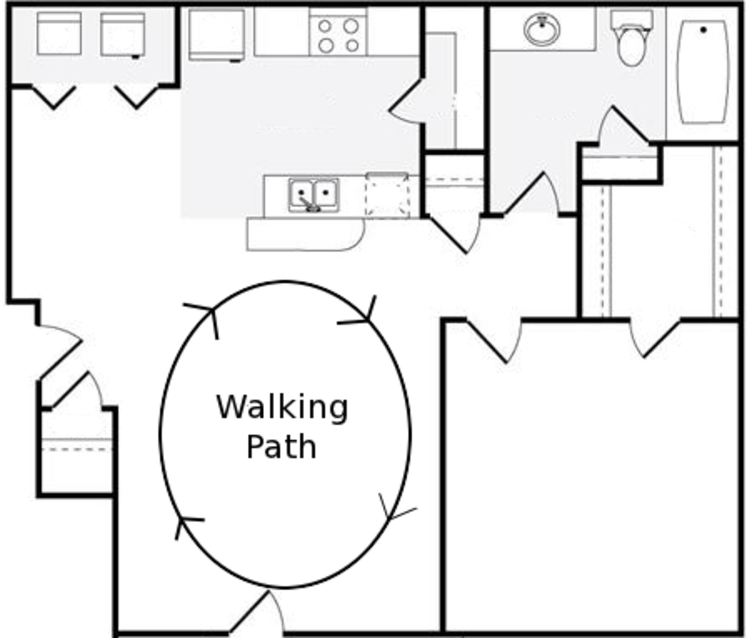
\includegraphics[width=0.6\textwidth]{figures/floorplan.pdf}
\end{center}
\caption{Walking environment.}
\label{fig:floorplan}
\end{figure}

\subsubsection{Cycle of Operations}\label{subsec:cycleofoperations}
A normal cycle of operations with $n$ devices works as follows:

\begin{algorithmic}[1]
\STATE AP sends synchronization beacon which includes routing and power control tables.
\STATE Each ED transmits its own RSSI table back to the AP, while simultaneously listening to other ED messages and storing the received power from each.
\STATE Once all EDs have transmitted their data, the AP sends a table with the RSSI data from all devices. (See Table~\ref{tab:rssi} for an example)
\STATE The host uses the RSSI table to compute the routes along with the required powers to meet the selected links.
\STATE The host sends both routing and power tables back to the AP so that a new cycle may begin.
\end{algorithmic}

\begin{table}[htb]
\begin{tabular}{|c|c|c|c|c|c|c|c|c|c|}
\hline  & AP & ED1 & ED2 & ED3 & ED4 & ED5 & ED6 & ED7 & ED8 \\ 
\hline AP & - & -60 & -60 & -60 & -60.5 & -60.5 & -60.5 & -60 & -79.5 \\ 
\hline ED1 & -66 & - & -62 & -75 & -63.5 & -69 & -75.5 & -73 & -67.5 \\ 
\hline ED2 & -72 & -61.5 & - & -80 & -69 & -70 & -74 & -75 & -66 \\ 
\hline ED3 & -77.5 & -74.5 & -80.5 & - & -67.5 & -70 & -72.5 & -70.5 & -70 \\ 
\hline ED4 & -39 & -63 & -69.5 & -67 & - & -82.5 & -74.5 & -69 & -65.5 \\ 
\hline ED5 & -67.5 & -68 & -71 & -69.5 & -84 & - & -55.5 & -51.5 & -62 \\ 
\hline ED6 & -67 & -75 & -75 & -72.5 & -75 & -55.5 & - & -44.5 & -53 \\ 
\hline ED7 & -46 & -70 & -77.5 & -70.5 & -69 & -50.5 & -45 & - & -51.5 \\ 
\hline ED8 & -78 & -67.5 & -66.5 & -71 & -66 & -62 & -54 & -51.5 & - \\ 
\hline 
\end{tabular} 
\caption{Sample RSSI Table}
\label{tab:rssi}
\end{table}


\subsubsection{Details}
To minimize the number of control packets from being transmitted, the EDs are not individually polled. The only control packet that is sent is the synchronization beacon, which also carries the routing and power tables. Once the EDs are synchronized, they transmit their data on a pre-defined schedule to avoid collisions. Each ED has a network ID ranging from 1 to $n$. The time between synchronization packets is divided into time-slots than are used by each ED. The time slot used depends on the network ID of each device. This removes the need to come up with time schedules during runtime.

The routing table is a simple array which lists the destination for each ED packet. The ED does not need to know the entire route its packets will take, but only next device in the path. Similarly, the power table lists the transmit power setting each device needs to use. The size of these tables is directly proportional to the number of devices in the network.

\begin{figure}[!htb]
\begin{center}
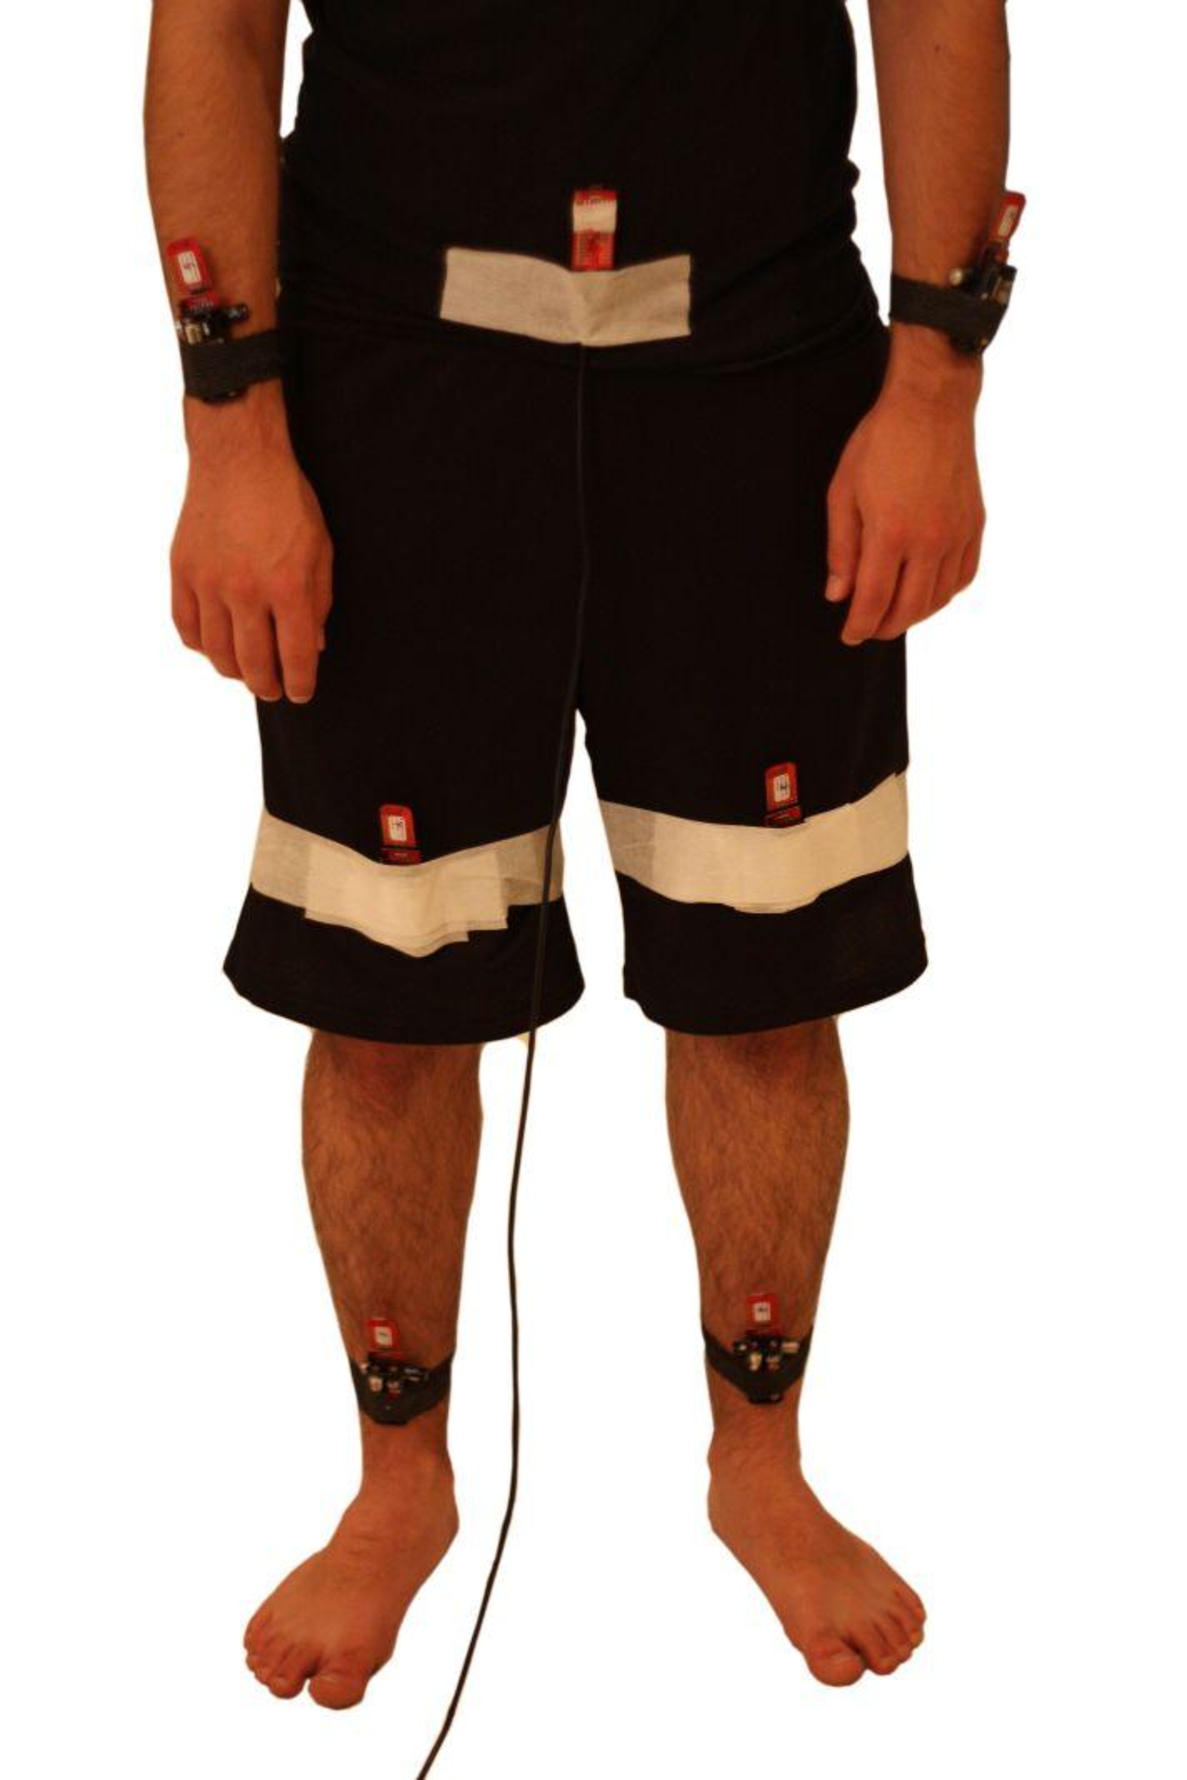
\includegraphics[width=0.6\textwidth]{figures/halfbody.pdf}
\end{center}
\caption{Subject with devices for RSSI capture}
\label{fig:halfbody}
\end{figure}


\subsection{Results}

Due to the similarities between the simulation and hardware implementation (they both use real RSSI data), the results were fairly similar. If fed with the same RSSI data, the algorithm will always produce the same results. The only difference with the hardware implementation is that the RSSI table is reduced due to the use of power control. Since each ED only uses enough transmit power to reach a specific ED, others might not receive the message. This was not a problem when the hardware experiment was run.

\begin{figure}[!ht]
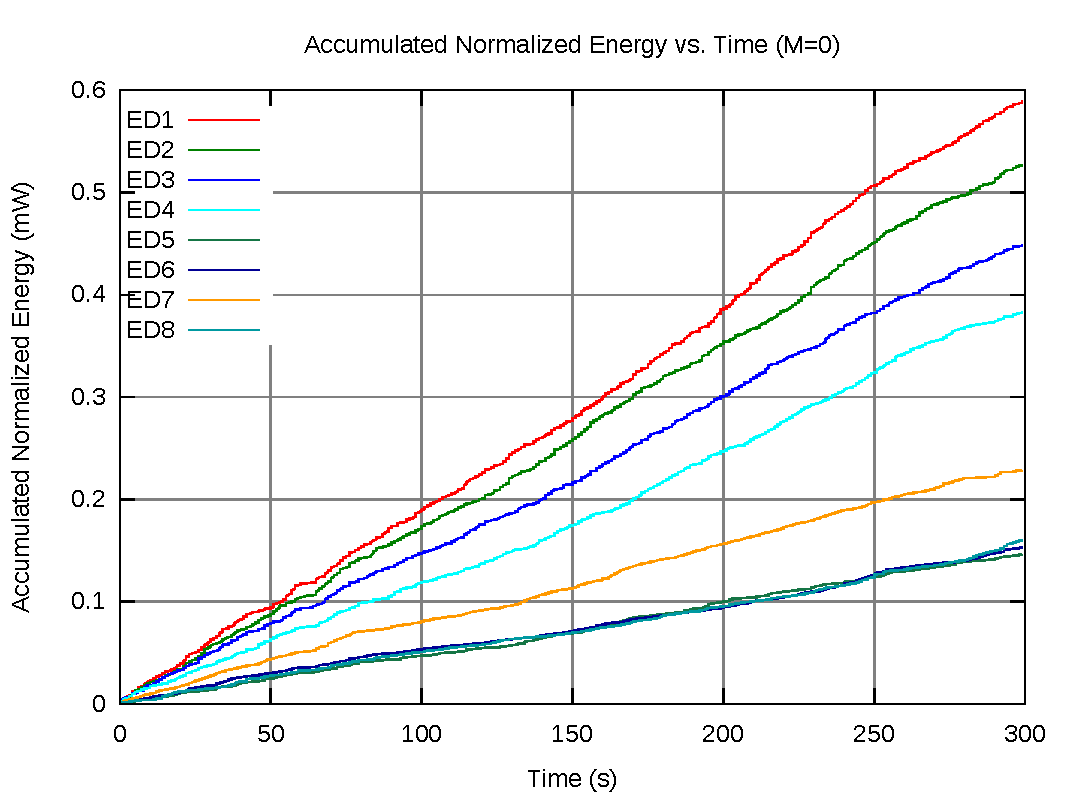
\includegraphics[width=0.8\textwidth]{figures/sit1-c0.pdf}
\caption{Sitting M=0}
\label{fig:sit1-c0}
\end{figure}

\begin{figure}[!ht]
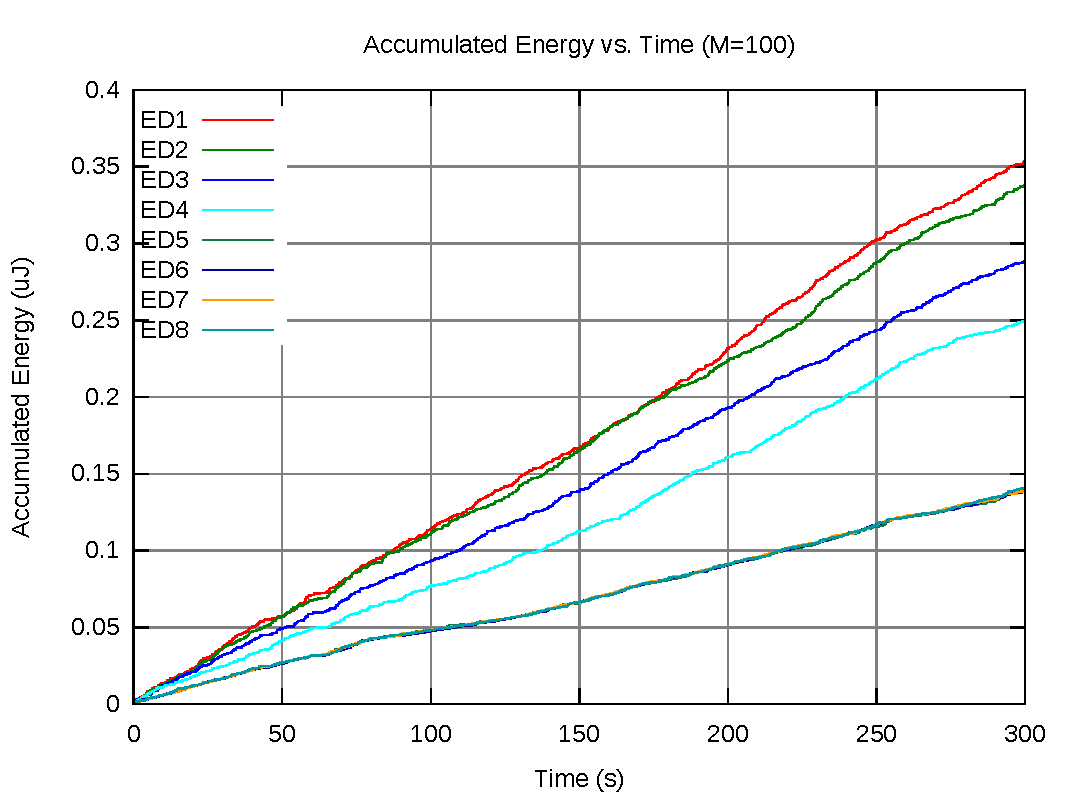
\includegraphics[width=0.8\textwidth]{figures/sit1-c100.pdf}
\caption{Sitting M=100}
\label{fig:sit1-c100}
\end{figure}

Figures~\ref{fig:sit1-c0}~and~\ref{fig:sit1-c100} show the resulting accumulated energies while the subject was in a sitting position. The experiment was run with both an $M=0$ as a reference, and $M=100$. Unfortunately, the results with a static subject were rather neutral. All EDs consume energy at different rates for both $M=0$ and $M=100$. A possible explanation for this is that the links between EDs remain close to the same as time passes. This can become a problem because certain EDs may only have a single path to choose from. If this is the case, they have no choice but to use the same link continuously. Not having a choice of paths impairs the ability of the routing algorithm to distribute energy use among all devices.

Figures~\ref{fig:walk2-c0}~and~\ref{fig:walk2-c100}, on the other hand, show an increase in network lifetime. For example, at the end of the 5 minute sampling run with $M=0$, the device which consumed the most power was ED7 with approximately 1.7 mW. On the other hand, with $M=100$, all EDs consume power in a uniform fashion and end up with less than 1.3 mW each. One important observation is that the network with $M=0$ consumed less overall power (~9.6mW) than the one with $M=100$ (~10.1mW). This is expected, due to the fact that the new cost function specifically avoids the most efficient path for a specific node in favor of the most efficient path for the whole network. While more energy is consumed overall, no single ED consumes significantly more power. 

To demonstrate the network lifetime improvement, an ED will be considered have depleted it's power source after consuming 1mW of normalized energy. In the previous example, the trial with $M=0$ reaches 1mW after approximately 175 seconds, while the case with $M=100$ reaches it around 240 seconds.

\begin{figure}[!ht]
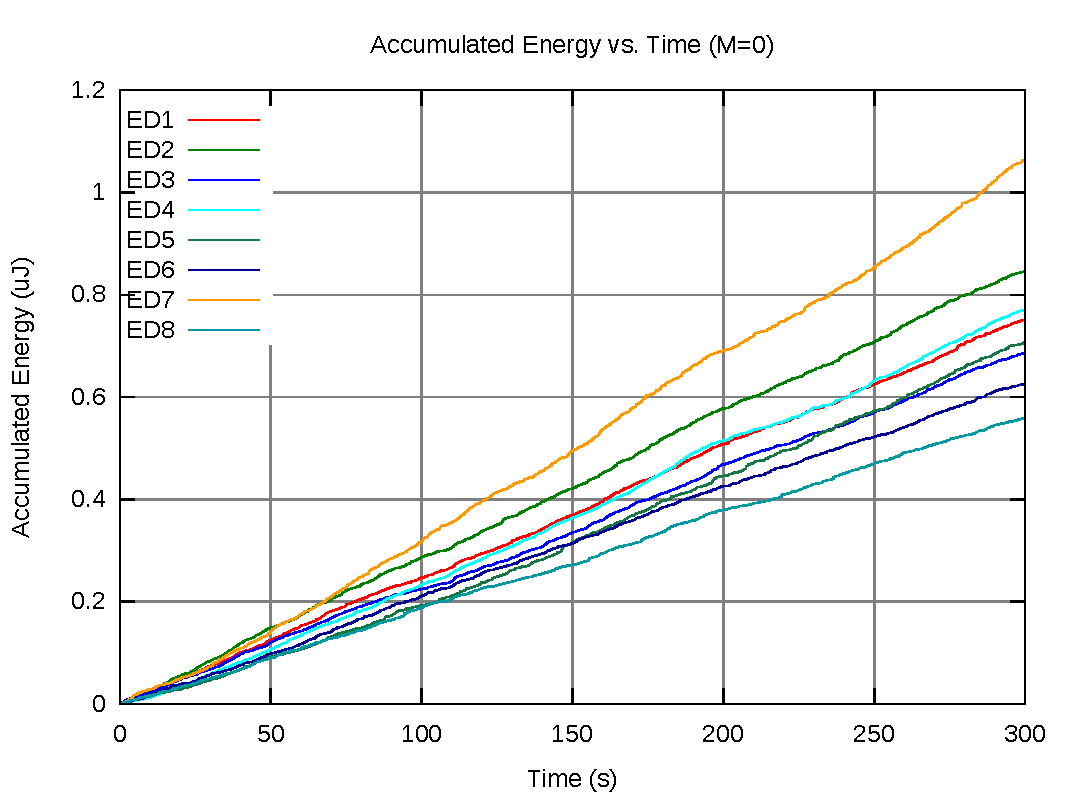
\includegraphics[width=0.8\textwidth]{figures/walk2-c0.pdf}
\caption{Walking M=0}
\label{fig:walk2-c0}
\end{figure}

\begin{figure}[!ht]
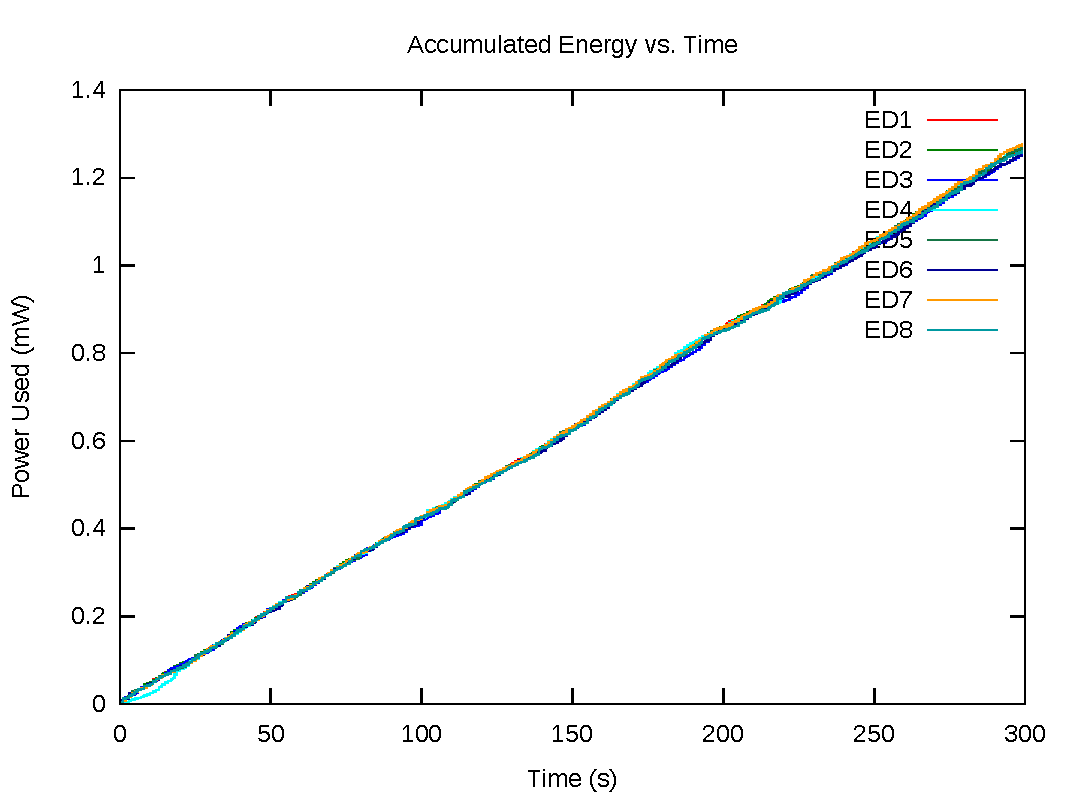
\includegraphics[width=0.8\textwidth]{figures/walk2-c100.pdf}
\caption{Walking M=100}
\label{fig:walk2-c100}
\end{figure}

A good example of the algorithm working was a result of hardware problems. During of the experiments, a single ED went off-line for several seconds and was manually restarted. Figure~\ref{fig:walk4-c100} shows the effect the ED failure had on the network. Because a device that is powered off does not consume power, it became the one with the least energy used. When it returned to the network, it was immediately used as a relay by other nodes.

\begin{figure}[!ht]
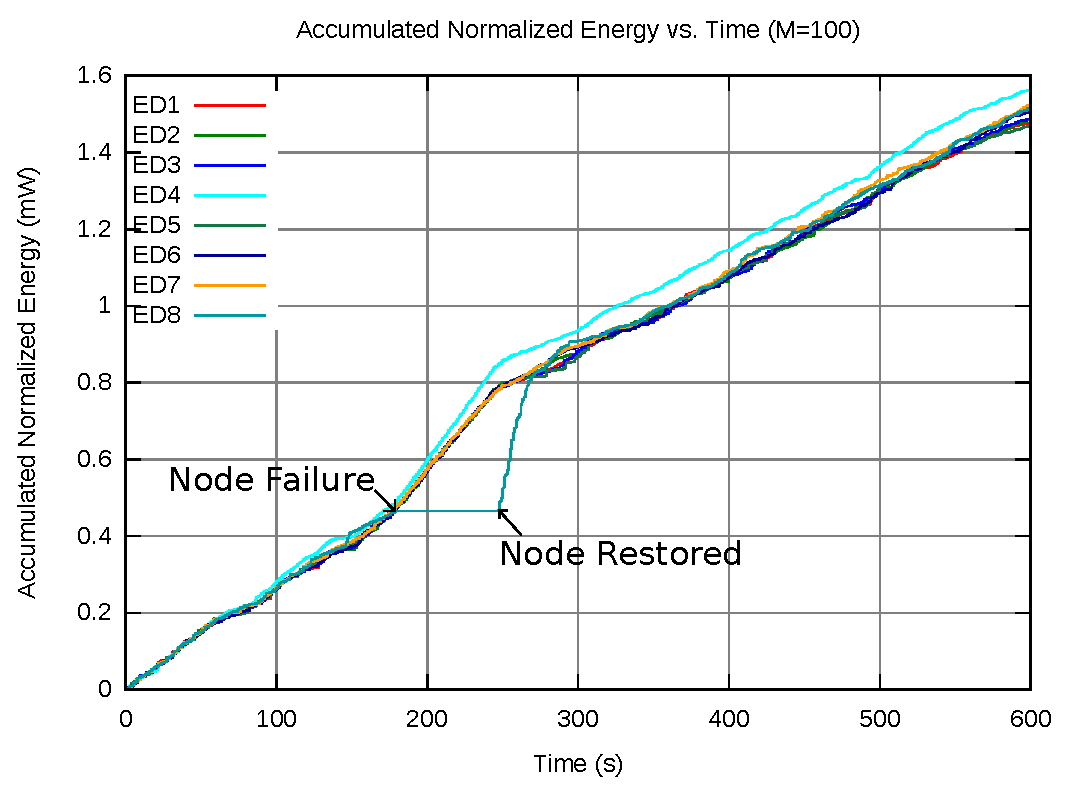
\includegraphics[width=0.8\textwidth]{figures/walk4-c100.pdf}
\caption{Walking M=100}
\label{fig:walk4-c100}
\end{figure}

\section{Conclusion}
The developed WBAN software libraries were successfully used to implement both the wireless ECG system and the full-body routing system. The wireless ECG system was able to sample data at a rate of 300Hz and display it in the host computer. The routing algorithm testing platform facilitated the development of the new link cost function to maximize network lifetime.

After analyzing the results, the new link cost function successfully improves network lifetime. The new cost function outperformed the traditional one in trials dealing with a dynamic environment, where the subject was walking. When the subject was not moving, both link costs performed about the same. Note that, in this case, performance is defined with respect to network lifetime, and not overall power consumption.

While the new link cost was successful, there is room for improvement. One improvement that can be done deals with the example from Figure~\ref{fig:walk4-c100}. While the failed ED was not part of the network, it was still taken into account when it came to link cost calculation. A better implementation would not include off-line devices in the calculation. A second modification would relate actual battery, or other power source, charge to the algorithm. This would allow for devices to join and leave the network while maintaining proper operation. It would also allow devices with different power sources to be included and used.

The use of power control, coupled with this new link cost function, should allow WBANs to run efficiently for long periods of time, while maximizing the network lifetime. Networks requiring all devices to be on-line to function will greatly benefit from this routing method. Other networks can also benefit. Due to the normalization of energy use in the network, devices will deplete their energy sources at similar times. This could be beneficial as all devices can be recharged or replaced simultaneously, instead of constantly monitoring and replacing individual devices.


\pagebreak

\listoffigures

%\listoftables

\bibliography{sources/thesis.bib}{}
\bibliographystyle{plain}
\end{document}